\documentclass[10pt,journal,twoside]{IEEEtran}

\usepackage[utf8]{inputenc}
\usepackage{amsmath,amsfonts,amssymb}
\usepackage{array}
\usepackage[table]{xcolor}
\usepackage{graphicx}
\usepackage{orcidlink}
\usepackage{multirow}
\usepackage{booktabs}
\usepackage{stfloats}
\usepackage{fancyhdr}
\hypersetup{
  colorlinks=true,
  linkcolor=blue,
  citecolor=blue,
  urlcolor=blue
}

\hyphenation{op-tical net-works semi-conduc-tor IEEE-Xplore audio-visual}
\raggedbottom
\setcounter{dbltopnumber}{4}
\renewcommand{\dbltopfraction}{0.95}
\renewcommand{\textfraction}{0.05}
\makeatletter
\setlength{\@dblfptop}{0pt}
\makeatother

\fancypagestyle{tmmfirst}{%
  \fancyhf{}
  \fancyhead[L]{\scriptsize IEEE TRANSACTIONS ON MULTIMEDIA}
  \fancyhead[R]{\scriptsize\thepage}
  \renewcommand{\headrulewidth}{0pt}}
\fancypagestyle{tmmrunning}{%
  \fancyhf{}
  \fancyhead[LO]{\scriptsize WANG et al.: SUPPLEMENTARY MATERIAL FOR KA-GZSL}
  \fancyhead[RE]{\scriptsize IEEE TRANSACTIONS ON MULTIMEDIA}
  \fancyhead[RO,LE]{\scriptsize\thepage}
  \renewcommand{\headrulewidth}{0pt}}
\pagestyle{tmmrunning}

\begin{document}

\title{Supplementary Material for\\
\textit{KA-GZSL: Knowledge-Guided Audio--Visual Generalized Zero-Shot Learning}}

\author{Hu~Wang, Jing~Yang, Xiaoli~Ruan, Yuling~Chen, Xinru~Yi, Chengjiang~Li, and Minyi~Guo}

\maketitle
\thispagestyle{tmmfirst}

% The main manuscript contains Tables I--IV; supplementary tables continue from V.
\setcounter{table}{4}
\setcounter{figure}{2}
\setcounter{equation}{27}

% This supplementary file contains multiple independent appendices.
\appendices

\newlength{\oldaboverulesep}
\newlength{\oldbelowrulesep}
\section{Additional Dataset and Implementation Details}

\subsection{Dataset Details}

\begin{table*}[!t]
  \centering
  \caption{Dataset splits for \text{VGGSound-GZSL}$^{\textit{cls}}$, \text{UCF-GZSL}$^{\textit{cls}}$, and \text{ActivityNet-GZSL}$^{\textit{cls}}$.}
  \label{tab:supp_dataset_split}
  \begin{tabular}{l c c c c c c @{\hspace{2em}} c c c}
    \toprule[1pt]
    \multirow{3}{*}{STAGE} & & & & \multicolumn{3}{c}{First stage} & \multicolumn{3}{c}{Second stage} \\
    \cmidrule(lr){5-7} \cmidrule(lr){8-10}
    & & & & Training & \multicolumn{2}{c}{Validation} & Training & \multicolumn{2}{c}{Test} \\
    \cmidrule(lr){5-5} \cmidrule(lr){6-7} \cmidrule(lr){8-8} \cmidrule(lr){9-10}
    DATASET & C & $\text{C}_\text{S}$ & $\text{C}_\text{U}$ & $\text{Tr}_\text{S}$ & $\text{Val}_\text{S}$ & $\text{Val}_\text{U}$ & $\text{Tr}_\text{S}$ & $\text{Te}_\text{S}$ & $\text{Te}_\text{U}$ \\
    \midrule[0.8pt]
    \text{UCF-GZSL}$^{\textit{cls}}$ & 51 & 30 & 21 & 30 & 30 & 12 & 42 & 42 & 9 \\
    \text{VGGSound-GZSL}$^{\textit{cls}}$ & 276 & 138 & 138 & 138 & 138 & 69 & 207 & 207 & 69 \\
    \text{ActivityNet-GZSL}$^{\textit{cls}}$ & 200 & 99 & 101 & 99 & 99 & 51 & 150 & 150 & 50 \\
    \bottomrule[1pt]
  \end{tabular}
\end{table*}

\textbf{\text{VGGSound-GZSL}}$^{\textit{cls}}$ is a modified version of the large-scale audio--visual dataset VGGSound. It contains a total of 276 classes, including 138 seen classes and 138 unseen classes. These classes can be roughly grouped into several major categories, such as animals, homes, music, nature, humans, sports, tools, vehicles, and others.

\textbf{\text{UCF-GZSL}}$^{\textit{cls}}$ is a subset of the UCF101 action recognition dataset. This dataset covers a wide range of daily activities, sports, and entertainment behaviors collected from YouTube. It consists of 51 classes, including 30 seen classes and 21 unseen classes. The categories include but are not limited to fencing, playing piano, dancing, and swimming.

\textbf{\text{ActivityNet-GZSL}}$^{\textit{cls}}$ is an action recognition dataset derived from ActivityNet that is specifically designed to support action recognition tasks. It contains 200 categories of daily activities, with more than 20,000 video clips and a total duration exceeding 849 hours. Each video clip in the dataset is accurately annotated with action categories and temporal boundaries, thus providing detailed data for training and evaluation.
Table~\ref{tab:supp_dataset_split} summarizes the class partitions under the two-stage protocol. Here, $C$, $C_\text{S}$, and $C_\text{U}$ denote all, seen, and unseen classes; $\text{Tr}_\text{S}$, $\text{Val}_\text{S}$, $\text{Val}_\text{U}$, $\text{Te}_\text{S}$, and $\text{Te}_\text{U}$ denote the corresponding training, validation, and test partitions.

\subsection{Implementation Details}

KA-GZSL is implemented in PyTorch and trained on a workstation with an Intel Core i9-14900KF CPU, 128~GB RAM, an NVIDIA GeForce RTX 3090~Ti GPU, and Ubuntu~24.04. Adam is used with a batch size of 64, weight decay $10^{-5}$, $\beta_1=0.9$, and $\beta_2=0.999$. The loss weights are $\alpha=0.5$, $\beta=0.7$, and $\varphi=0.5$. Initial learning rates are $10^{-4}$, $7\times10^{-5}$, and $10^{-4}$ for \text{VGGSound-GZSL}$^{\textit{cls}}$, \text{UCF-GZSL}$^{\textit{cls}}$, and \text{ActivityNet-GZSL}$^{\textit{cls}}$, respectively. The learning rate is multiplied by 0.1 when validation HM does not improve for three consecutive epochs. Stage-one training uses 15 epochs for \text{VGGSound-GZSL}$^{\textit{cls}}$ and \text{ActivityNet-GZSL}$^{\textit{cls}}$ and 20 epochs for \text{UCF-GZSL}$^{\textit{cls}}$.

The two-stage protocol uses the stage-one validation classes as pseudo-unseen classes to select the calibrated-stacking parameter and epoch count. Stage two retrains on the union of the original training and validation sets. The final test-unseen classes $\mathrm{Te}_{U}$ remain disjoint from all audio--visual samples used for training. The trained stage-two model is then applied to the test set, and the other experimental settings follow ClipClap-GZSL as stated in the main manuscript.

\section{LLM Prompting and Semantic Description Details}

For a category name \{category\}, the recorded modality-specific templates are ``a photo of a person doing \{category\}'' for visual semantics and ``a person doing \{category\} can be heard'' for audio semantics. The class explanation is elicited by an instruction of the form ``Please provide a detailed explanation of the body movements involved in \{category\}.'' As defined in Eq.~(1) of the main manuscript, the generated explanation is concatenated with the corresponding modality-specific template before text encoding. The corresponding prompt ablation is reported in Table~III of the main manuscript.

% AUTHOR INPUT REQUIRED BEFORE SUBMISSION: record the actual LLM model/version,
% access date, decoding parameters, post-processing, and human verification protocol.

\section{Extended Ablation Studies}

\subsection{Influence of Different Training Losses}

\begin{table*}[!t]
  \centering
  \caption{Influence of different training losses.}
  \label{tab:supp_loss_ablation}
  \begin{tabular}{c cccc c cccc c cccc}
    \toprule[2pt]
    \multirow{2}{*}{\textbf{Loss}}
    & \multicolumn{4}{c}{\textbf{\text{VGGSound-GZSL}}$^{\textit{cls}}$} & & \multicolumn{4}{c}{\textbf{\text{UCF-GZSL}}$^{\textit{cls}}$} & & \multicolumn{4}{c}{\textbf{\text{ActivityNet-GZSL}}$^{\textit{cls}}$} \\
    \cmidrule(lr){2-5} \cmidrule(lr){7-10} \cmidrule(lr){12-15}
    & S & U & HM & ZSL & & S & U & HM & ZSL & & S & U & HM & ZSL \\
    \midrule[1pt]
    w/o $L_n$ & 6.23 & 7.98 & 7.00 & 7.95 & & 20.23 & 15.23 & 17.38 & 18.14 & & 9.31 & 7.45 & 8.28 & 14.95 \\
    w/o $L_p$ & 16.42 & 6.24 & 9.04 & \textbf{12.77} & & 65.72 & 19.49 & 30.06 & 25.48 & & 19.65 & 11.26 & 14.32 & 15.49 \\
    w/o $L_c$ & 19.54 & 6.98 & 10.29 & 7.32 & & 69.54 & 23.58 & 35.22 & 23.96 & & 26.12 & 16.55 & 20.26 & 12.97 \\
    \noalign{\global\setlength{\oldaboverulesep}{\aboverulesep}}
    \noalign{\global\setlength{\oldbelowrulesep}{\belowrulesep}}
    \noalign{\global\setlength{\aboverulesep}{0pt}}
    \noalign{\global\setlength{\belowrulesep}{1.5pt}}
    \midrule[1pt]
    \rowcolor{gray!25}
    \textbf{$L$} & \textbf{32.47} & \textbf{11.28} & \textbf{16.74} & 12.16 & & \textbf{83.79} & \textbf{46.68} & \textbf{59.96} & \textbf{48.98} & & \textbf{42.80} & \textbf{23.18} & \textbf{30.07} & \textbf{24.24} \\
    \bottomrule[2pt]
    \noalign{\global\setlength{\aboverulesep}{\oldaboverulesep}}
    \noalign{\global\setlength{\belowrulesep}{\oldbelowrulesep}}
  \end{tabular}
\end{table*}

Table~\ref{tab:supp_loss_ablation} shows that the complete loss yields the highest HM on all three datasets. Removing $L_n$ reduces \text{UCF-GZSL}$^{\textit{cls}}$ HM/ZSL from 59.96\%/48.98\% to 17.38\%/18.14\% and \text{VGGSound-GZSL}$^{\textit{cls}}$ HM from 16.74\% to 7.00\%. Removing $L_p$ or $L_c$ lowers \text{ActivityNet-GZSL}$^{\textit{cls}}$ HM from 30.07\% to 14.32\% or 20.26\%, respectively. These results confirm that all three loss terms are necessary for balanced performance.


\subsection{Influence of Different Text Encoders on the Construction of the Knowledge Graph}

\begin{table*}[!t]
  \centering
  \caption{Influence of different text encoders on knowledge graph construction.}
  \label{tab:supp_text_encoder}
  \begin{tabular}{c cccc c cccc c cccc}
    \toprule[2pt]
    \multirow{2}{*}{\textbf{Text Encoder}}
    & \multicolumn{4}{c}{\text{VGGSound-GZSL}$^{\textit{cls}}$} & & \multicolumn{4}{c}{\text{UCF-GZSL}$^{\textit{cls}}$} & & \multicolumn{4}{c}{\text{ActivityNet-GZSL}$^{\textit{cls}}$} \\
    \cmidrule(lr){2-5} \cmidrule(lr){7-10} \cmidrule(lr){12-15}
    & S & U & HM & ZSL & & S & U & HM & ZSL & & S & U & HM & ZSL \\
    \midrule[1pt]
    CLIP & 30.55 & 9.71 & 14.74 & 10.62 & & 79.82 & 34.67 & 48.34 & 39.81 & & 40.63 & 22.40 & 28.88 & 23.86 \\
    CLAP & 21.34 & 9.52 & 13.17 & 9.73 & & 59.77 & 42.46 & 49.65 & 40.36 & & 37.04 & 15.95 & 22.30 & 19.54 \\
    \noalign{\global\setlength{\oldaboverulesep}{\aboverulesep}}
    \noalign{\global\setlength{\oldbelowrulesep}{\belowrulesep}}
    \noalign{\global\setlength{\aboverulesep}{0pt}}
    \noalign{\global\setlength{\belowrulesep}{1.5pt}}
    \midrule[1pt]
    \rowcolor{gray!25}
    \textbf{Both} & \textbf{32.47} & \textbf{11.28} & \textbf{16.74} & \textbf{12.16} & & \textbf{83.79} & \textbf{46.68} & \textbf{59.96} & \textbf{48.98} & & \textbf{42.80} & \textbf{23.18} & \textbf{30.07} & \textbf{24.24} \\
    \bottomrule[2pt]
    \noalign{\global\setlength{\aboverulesep}{\oldaboverulesep}}
    \noalign{\global\setlength{\belowrulesep}{\oldbelowrulesep}}
  \end{tabular}
\end{table*}

Table~\ref{tab:supp_text_encoder} compares CLIP-only, CLAP-only, and joint text encoding for knowledge-graph construction. Joint encoding achieves HM scores of 16.74\%, 59.96\%, and 30.07\% on \text{VGGSound-GZSL}$^{\textit{cls}}$, \text{UCF-GZSL}$^{\textit{cls}}$, and \text{ActivityNet-GZSL}$^{\textit{cls}}$, respectively, outperforming either single encoder on every dataset. For example, the CLIP-only and CLAP-only HM scores are 14.74\% and 13.17\% on \text{VGGSound-GZSL}$^{\textit{cls}}$ and 48.34\% and 49.65\% on \text{UCF-GZSL}$^{\textit{cls}}$. ZSL follows the same trend, indicating that CLIP and CLAP provide complementary visual and auditory semantic priors.

\subsection{Influence of the Weighting Coefficients \texorpdfstring{$\alpha$, $\beta$, and $\varphi$}{alpha, beta, and phi} in the Loss Function}

\begin{table*}[!t]
  \centering
  \caption{Influence of weighting coefficients $\alpha$, $\beta$, and $\varphi$ in the loss function.}
  \label{tab:supp_loss_coeff}
  \begin{tabular}{ccc cccc c cccc c cccc}
    \toprule[2pt]
    \multicolumn{3}{c}{\multirow{2}{*}{\textbf{Factor}}}
    & \multicolumn{4}{c}{\text{VGGSound-GZSL}$^{\textit{cls}}$} & & \multicolumn{4}{c}{\text{UCF-GZSL}$^{\textit{cls}}$} & & \multicolumn{4}{c}{\text{ActivityNet-GZSL}$^{\textit{cls}}$} \\
    \cmidrule(lr){4-7} \cmidrule(lr){9-12} \cmidrule(lr){14-17}
    $\alpha$ & $\beta$ & $\varphi$ & S & U & HM & ZSL & & S & U & HM & ZSL & & S & U & HM & ZSL \\
    \midrule[1pt]
    $\times$ & $\times$ & $\times$ & 23.53 & 5.68 & 9.15 & 6.94 & & 56.38 & 30.45 & 39.54 & 25.68 & & 27.04 & 12.73 & 17.31 & 15.64 \\
    $\times$ & $\checkmark$ & $\checkmark$ & 24.72 & 6.86 & 10.74 & 7.55 & & 69.57 & 39.72 & 50.57 & 38.98 & & 31.29 & 18.94 & 23.60 & 17.44 \\
    $\checkmark$ & $\times$ & $\checkmark$ & 28.55 & 7.27 & 11.59 & 9.13 & & 74.94 & \textbf{49.92} & 59.92 & 42.64 & & 35.71 & 17.59 & 23.57 & 20.43 \\
    $\checkmark$ & $\checkmark$ & $\times$ & 28.93 & 6.38 & 10.45 & 8.97 & & 68.45 & 42.98 & 52.80 & 41.75 & & 40.85 & 20.67 & 27.45 & \textbf{24.76} \\
    \noalign{\global\setlength{\oldaboverulesep}{\aboverulesep}}
    \noalign{\global\setlength{\oldbelowrulesep}{\belowrulesep}}
    \noalign{\global\setlength{\aboverulesep}{0pt}}
    \noalign{\global\setlength{\belowrulesep}{1.5pt}}
    \midrule[1pt]
    \rowcolor{gray!25}
    \textbf{$\checkmark$} & \textbf{$\checkmark$} & \textbf{$\checkmark$} & \textbf{32.47} & \textbf{11.28} & \textbf{16.74} & \textbf{12.16} & & \textbf{83.79} & 46.68 & \textbf{59.96} & \textbf{48.98} & & \textbf{42.80} & \textbf{23.18} & \textbf{30.07} & 24.24 \\
    \bottomrule[2pt]
    \noalign{\global\setlength{\aboverulesep}{\oldaboverulesep}}
    \noalign{\global\setlength{\belowrulesep}{\oldbelowrulesep}}
  \end{tabular}
\end{table*}

Table~\ref{tab:supp_loss_coeff} evaluates the weighting coefficients in Eq.~(27) of the main manuscript. Using $\alpha$, $\beta$, and $\varphi$ jointly yields the highest HM on all three datasets, although individual S, U, or ZSL values need not be maximal. Removing $\alpha$ lowers \text{UCF-GZSL}$^{\textit{cls}}$ HM by 9.39 percentage points, removing $\beta$ lowers \text{ActivityNet-GZSL}$^{\textit{cls}}$ HM by 6.50 points, and removing $\varphi$ lowers \text{VGGSound-GZSL}$^{\textit{cls}}$ HM by 6.29 points. Thus, the three weights complementarily balance $L_n$, $L_p$, and $L_c$.

\section{Additional Qualitative Analysis}

\begin{figure*}[!t]
  \centering
  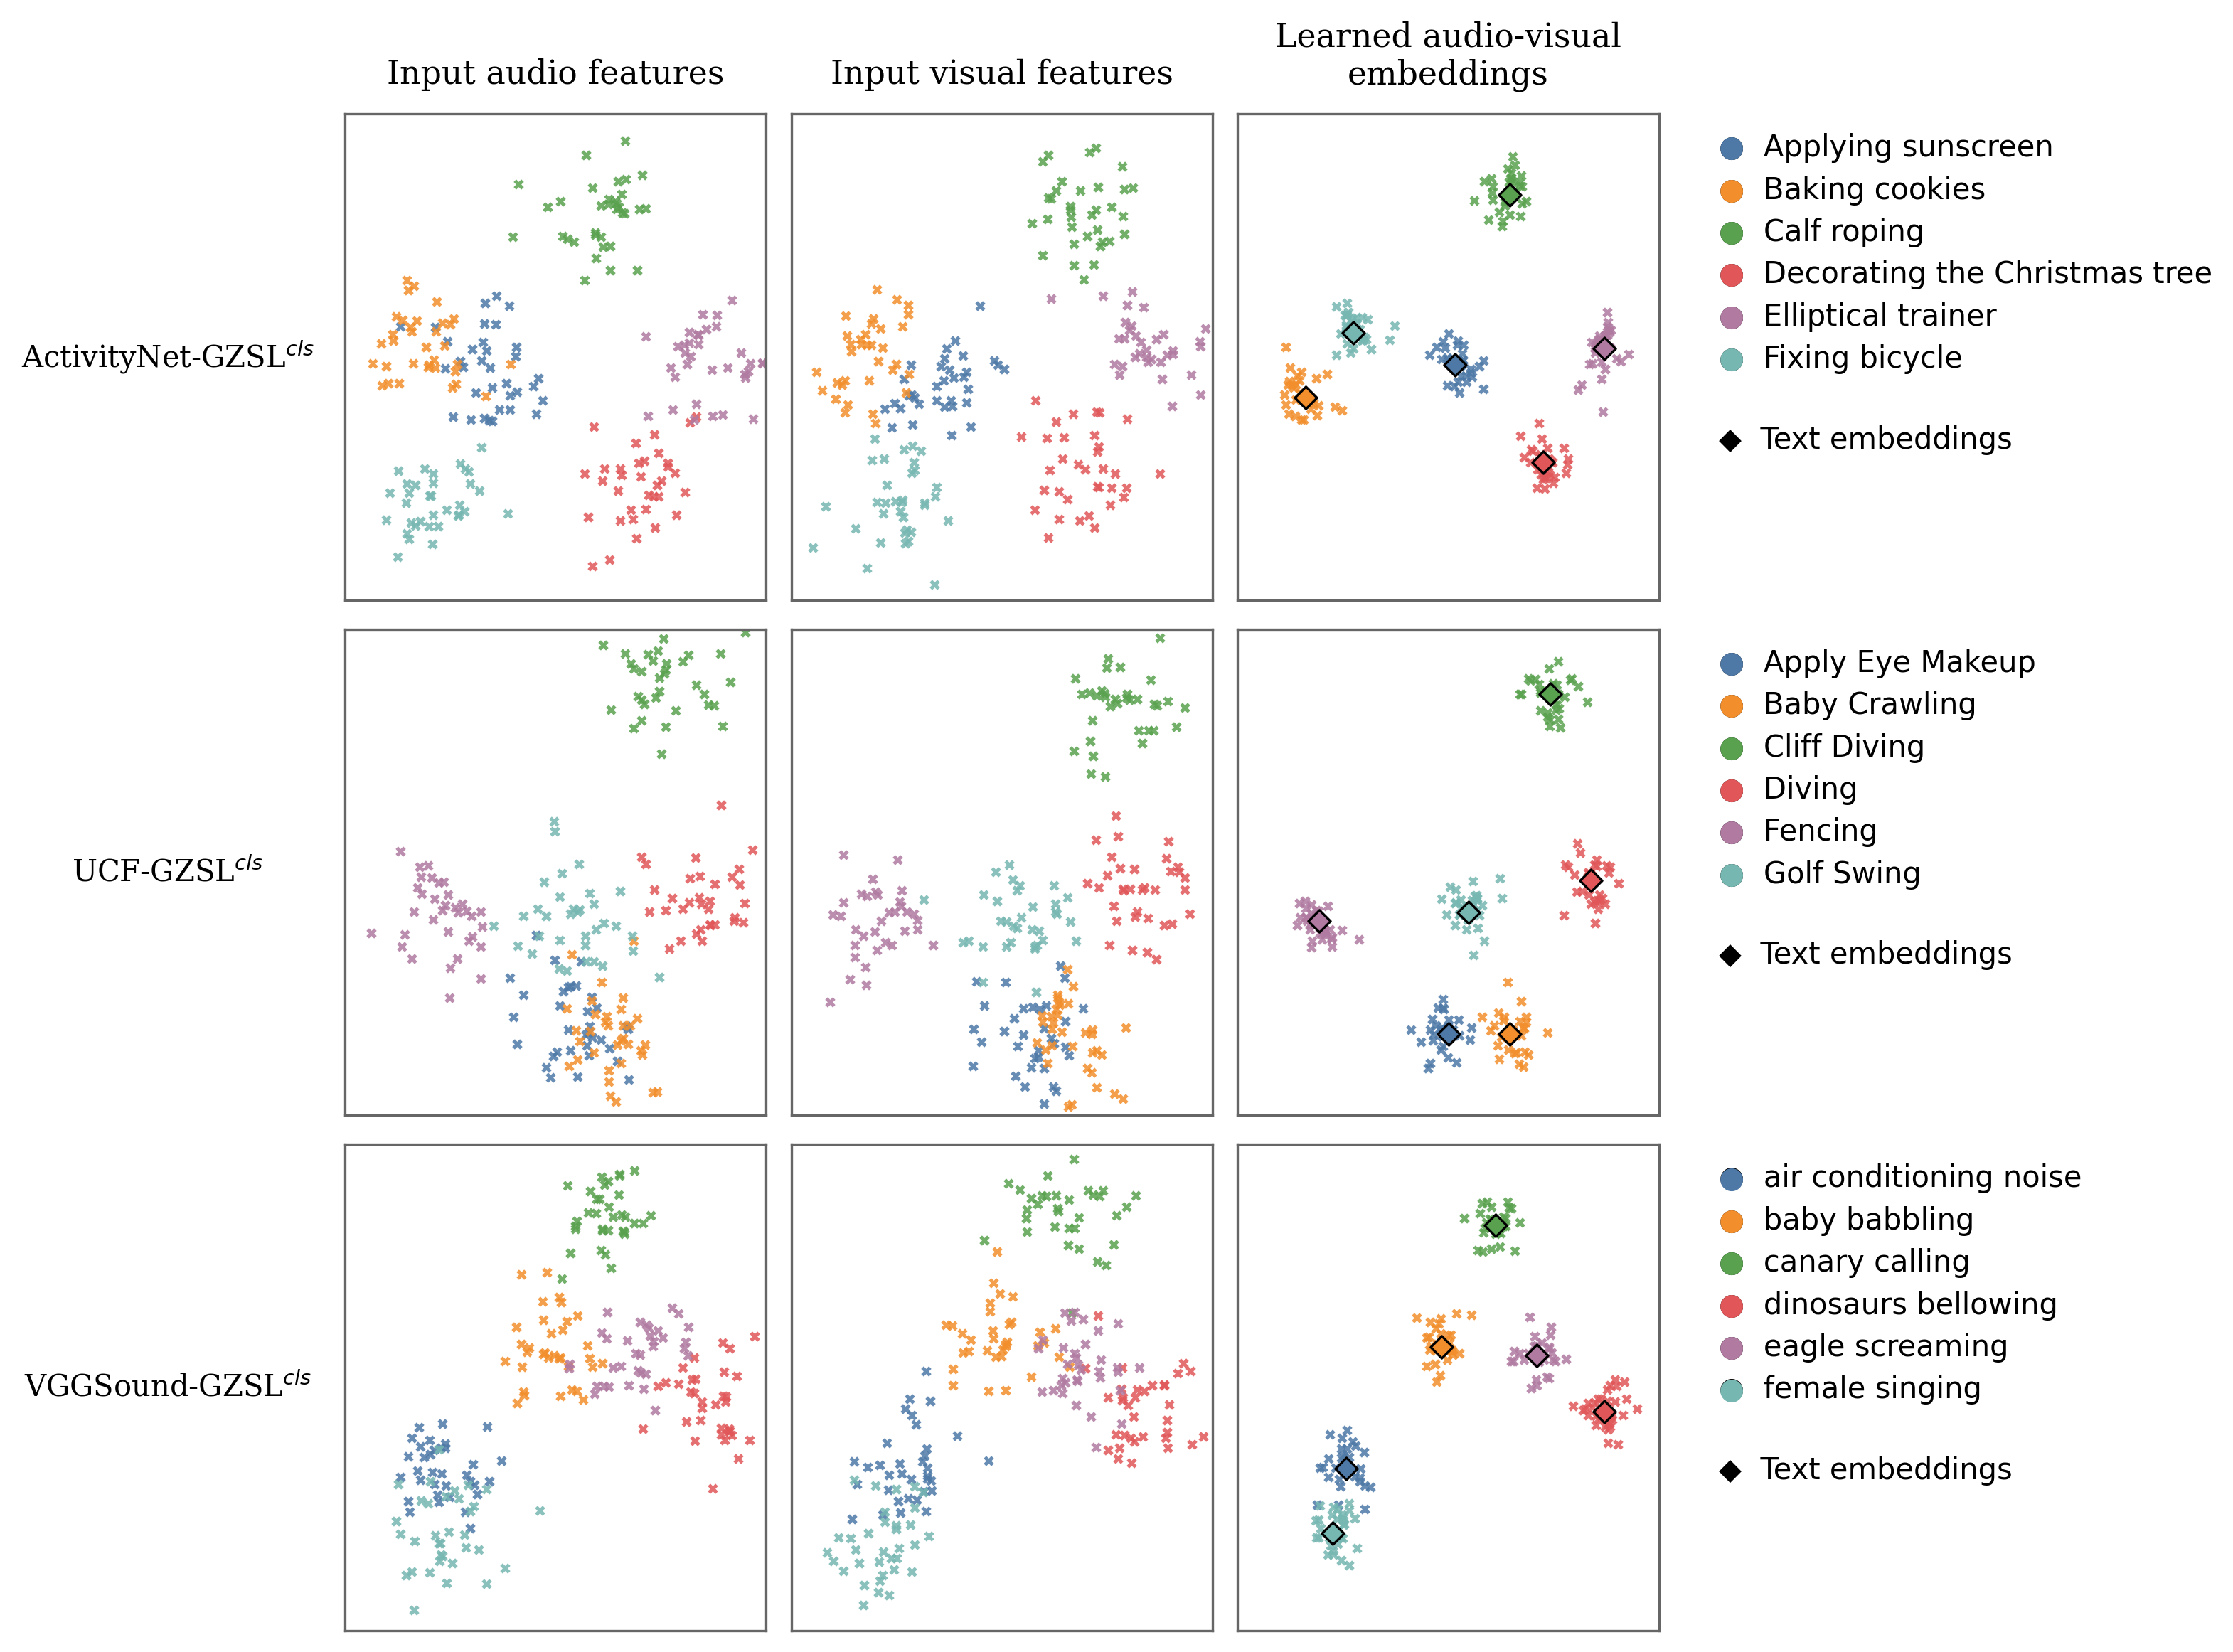
\includegraphics[width=0.94\textwidth]{figure/tsne.png}
  \caption{t-SNE visualization on \text{VGGSound-GZSL}$^{\textit{cls}}$, \text{UCF-GZSL}$^{\textit{cls}}$, and \text{ActivityNet-GZSL}$^{\textit{cls}}$. Columns show raw audio features, raw visual features, and learned joint audio--visual embeddings for six classes. Black diamonds denote the corresponding class-semantic embeddings.}
  \label{fig:supp_tsne}
\end{figure*}

Figure~\ref{fig:supp_tsne} presents the audio input features (left), visual input features (center), and joint audio--visual embeddings learned by KA-GZSL (right) for six classes from \text{VGGSound-GZSL}$^{\textit{cls}}$, \text{UCF-GZSL}$^{\textit{cls}}$, and \text{ActivityNet-GZSL}$^{\textit{cls}}$. The raw audio and visual features are relatively dispersed and have less distinct class boundaries, whereas the learned joint embeddings form more compact and separable clusters. Moreover, the class-semantic embeddings, shown as black diamonds, lie within their corresponding audio--visual clusters. These observations qualitatively support the alignment between the learned multimodal representations and their class semantics.

\end{document}
